\documentclass[10pt, a5paper]{article}
\usepackage{pdfpages}
\usepackage{parallel}
\usepackage[T2A]{fontenc}
\usepackage{ucs}
\usepackage[utf8x]{inputenc}
\usepackage[polish,english,russian]{babel}
\usepackage{hyperref}
\usepackage{rotating}
\usepackage[inner=2cm,top=1.8cm,outer=2cm,bottom=2.3cm,nohead]{geometry}
\usepackage{listings}
\usepackage{graphicx}
\usepackage{wrapfig}
\usepackage{longtable}
\usepackage{indentfirst}
\usepackage{array}
\newcolumntype{P}[1]{>{\raggedright\arraybackslash}p{#1}}
\frenchspacing
\usepackage{fixltx2e} %text sub- and superscripts
\usepackage{icomma} % коскі ў матэматычным рэжыме
\PreloadUnicodePage{4}

\newcommand{\longpage}{\enlargethispage{\baselineskip}}
\newcommand{\shortpage}{\enlargethispage{-\baselineskip}}

\def\switchlang#1{\expandafter\csname switchlang#1\endcsname}
\def\switchlangbe{
\let\saverefname=\refname%
\def\refname{Літаратура}%
\def\figurename{Іл.}%
}
\def\switchlangen{
\let\saverefname=\refname%
\def\refname{References}%
\def\figurename{Fig.}%
}
\def\switchlangru{
\let\saverefname=\refname%
\let\savefigurename=\figurename%
\def\refname{Литература}%
\def\figurename{Рис.}%
}

\hyphenation{admi-ni-stra-tive}
\hyphenation{ex-pe-ri-ence}
\hyphenation{fle-xi-bi-li-ty}
\hyphenation{Py-thon}
\hyphenation{ma-the-ma-ti-cal}
\hyphenation{re-ported}
\hyphenation{imp-le-menta-tions}
\hyphenation{pro-vides}
\hyphenation{en-gi-neering}
\hyphenation{com-pa-ti-bi-li-ty}
\hyphenation{im-pos-sible}
\hyphenation{desk-top}
\hyphenation{elec-tro-nic}
\hyphenation{com-pa-ny}
\hyphenation{de-ve-lop-ment}
\hyphenation{de-ve-loping}
\hyphenation{de-ve-lop}
\hyphenation{da-ta-ba-se}
\hyphenation{plat-forms}
\hyphenation{or-ga-ni-za-tion}
\hyphenation{pro-gramming}
\hyphenation{in-stru-ments}
\hyphenation{Li-nux}
\hyphenation{sour-ce}
\hyphenation{en-vi-ron-ment}
\hyphenation{Te-le-pathy}
\hyphenation{Li-nux-ov-ka}
\hyphenation{Open-BSD}
\hyphenation{Free-BSD}
\hyphenation{men-ti-on-ed}
\hyphenation{app-li-ca-tion}

\def\progref!#1!{\texttt{#1}}
\renewcommand{\arraystretch}{2} %Іначай формулы ў матрыцы зліпаюцца з лініямі
\usepackage{array}

\def\interview #1 (#2), #3, #4, #5\par{

\section[#1, #3, #4]{#1 -- #3, #4}
\def\qname{LVEE}
\def\aname{#1}
\def\q ##1\par{{\noindent \bf \qname: ##1 }\par}
\def\a{{\noindent \bf \aname: } \def\qname{L}\def\aname{#2}}
}

\def\interview* #1 (#2), #3, #4, #5\par{

\section*{#1\\{\small\rm #3, #4. #5}}

\def\qname{LVEE}
\def\aname{#1}
\def\q ##1\par{{\noindent \bf \qname: ##1 }\par}
\def\a{{\noindent \bf \aname: } \def\qname{L}\def\aname{#2}}
}

\switchlang{be}
\begin{document}
\title{Досвед апрацоўкі відэа з дакладаў ці лекцый з дапамогай kdenlive\footnote{\url{andrej@zahar.ws}, \url{http://lvee.org/ru/abstracts/234}}}
\author{Андрэй Захарэвіч, Мiнск, Беларусь}
\maketitle
\begin{abstract}
This thesis contains some background ideas for my workshop. Workshop will demonstrates one of the ways of video processing some content from presentations, lectures and so one using \linebreak Kdenlive, the open-source multitrack video editor.
\end{abstract}
\section*{Прадмова}

Тэзісы ніжэй фактычна фіксуюць некалькі думак і назіранняў, тлумачаць чаму для мантажа відэа для лінукосвак я выбраў гэты інструмент (kdenlive) і менавіта такі фармат. Для таго каб зразумець воркшоп не абавязковыя, але могуць быць карысныя тым, хто шукае свае інструменты і падыходы для працы з гэткім кантэнтам.

\section*{З чаго пачыналася}

Пачыналі мы, як і большасць, я думаю, з таго што пачалі запісваць відэа. То бок ёсць праекцыйная дошка, побач з якой умоўна кажучы лектар і гэта ўсё фіксуецца камерай~\cite{Zakharevich1}.


\begin{figure}[h!]
  \centering
  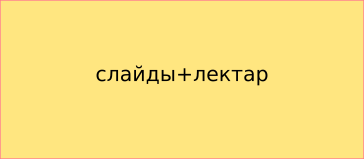
\includegraphics[width=8cm]{32_2016_Zakharevich1.png}
\end{figure}

На гэтым жа месцы і сустрэлі першыя граблі: калі не ставіць спецыяльнае святло, то лектар значна больш слаба падсвечваецца чым экран, на які праектар паказвае слайды. І тут альбо зыркі экран у чорнай рамцы, дзе вяла варушыцца цень лектрара, альбо лектар, які стаіць побач з невыносна зыркім экранам, глядзець які немагчыма. Часцей за ўсё нешта невыноснай якасці паміж гэтымі крайнасцямі. А калі дадаць усякія іншыя эфекты такой разнасці святла ў кадры, кшталту шума і іншага, то ясна: тут не тое што лектара ўбачыць, тут хаця б самыя вялікія літаркі на слайдзе прачытаць бы.

Аднойчы Wargaming прапанаваў нам здымаць даклады на лінуксоўках сваёй (прафесійнай) тэхнікай, і каб гэты матэрыял апрацоўвалі спецыялісты. Адрозненні пачаліся ад пачатку: прафесіяналы вырашылі праблему з тым што нешта нечытаецца не толькі камерай лепшай якасці, але і правільна пастаўленым святлом. Выніковае відэа атрымалася значна лепш, усё чыталася, разгубленыя твары дакладчыкаў было добра бачна ў кадры.

Чаму разгубленыя? А гэта другая праблема падыхода ``здымаем слайды і дакладчыка адной камерай'', для тых хто прайшоў першы ўзровень квеста і выставіў святло: дакладчык не бачыць аўдыторыі. Для яго няма слухачоў, ён бачыць толькі святло ў твар і цемру за лямпай.

Гэта можа не быць праблемай, калі вы здымаеце нейкую акадэмічную канферэнцыю ці паточную лекцыю, дзе узаемадзеяння паміж слухачамі і лектарам не прадугледжана. І, тым не меньш, большасць знаёмых лектараў і дакладчыкаў хочуць бачыць рэакцыю аўдыторыі на свае словы. Не кажучы пра тое, што для дакладаў у фармаце лінуксовак, калі можна задаваць пытанні практычна ў любы момант ці дапаўняць дакладчыка, гэта сапраўдная катастрофа.

\section*{Які фармат больш падыходзіць?}

Адказ відавочны: слайды павінны займаць большую частку \linebreak плошчы кадра і побач было б неблага каб мітусіўся лектар (для таго каб крыху больш цікава было глядзець). Слайды павінны быць у такой якасці, каб весь без выключэння тэкст чытаўся~\cite{Zakharevich2}. Гэта асноўнае, усялякія дадаткі пра тое што яшчэ можа быць "--- крыху ніжэй.

\begin{figure}[h!]
  \centering
  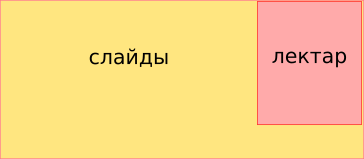
\includegraphics[width=8cm]{32_2016_Zakharevich2.png}
\end{figure}

Я сустракаў такое відэа, але мне здавалася, што гэта неверагодна складана і робіцца не нейкіх пакетах, якія вывучыць за пару вечароў неўважлівага гартання даведкі і спроб немагчыма. Трэба быць прафесіяналам і лепш яшчэ і са стажам, вышэйшай адукацыяй і заробкам, які група энтузіястаў проста не ў стане будзе сабраць.

Крокам наперад стала калі я пазнаёміўся з распрацоўкай Стафа Фаміна (Масква, РФ) якая называецца SeminarAssembler~\cite{Zakharevich3}. Вельмі раю азнаёміцца з відэакіраўніцтвамі і іншымі матэрыяламі па спасылцы, яны моцна прачышчаюць мозг і падштурхваюць да разумення што галоўнае.

А галоўнае, вядома ж, слайды, або дэманстрацыя чагосьці праз праектар і яны павінны займаць асноўнае месца у кадры. Неблага, калі побач са слайдамі бачна дакладчыка. Бо гэта атрымаліваецца неяк больш асабіста і цікава. Дапамагае не заснуць падчас лекцыі, што ў любым навучальным працэсе безумоўны плюс. Каб дадаць інтэрактыву можна ставіць недзе побач яшчэ і аўдыторыю, каб слухач адчуваў сябе часткай групы. Зноўку ж, дапамагае засяродзіцца. Хаця і ужо зусім неабавязкова.

\begin{figure}[h!]
  \centering
  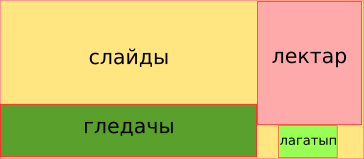
\includegraphics[width=8cm]{32_2016_Zakharevich3.png}
\end{figure}

З неабавязковых, але прыемных рэчаў можна яшчэ успомніць, напрыклад, лагатып, які зойме пустое месца на вольнай ад сэнсу частцы кадра фінальнага відэа. І калі дакладчык не паклапаціўся ўставіць гэта ў слайды, то небгала на пачатку даць назву даклада і імя (а можа і кантакты) дакладчыка.

\section*{Як атрымаць патрэбнае}

Усё вышэйузгаданае SeminarAssembler выдатна умее, больш за тое: апрацоўка скрыптуецца, дзяленне на часткі задаецца зручна, плюс разумныя патрабванні да жалеза (яно не аджырае жалеза пад свае задачы, пакідаючы на відэаапрацоўку, што вельмі карысна), выкарыстоўвае добра вядомыя сродкі апрацоўкі, не ствараючы сваіх веласіпедаў і нават мае свабодныя зыходнікі~\cite{Zakharevich4}, плюс дакументацыя і відэакіраўніцтва~\cite{Zakharevich3}.

Здавалася б, вось яно: ідэальны сродак для апрацоўкі відэа існуе. Але ёсць адзін дробны мінус, які для мяне асабіста ламае ўсё гэтае шчасце: гэта праграма працуе выключна пад Windows. Ставіць віртуалку для такой прагнай да рэсурсаў задачы "--- глупства. Трымаць асобны кампьютэр пад адну задачу "--- немагчыма. Можна, канешне, зрабіць дуалбут, але: крыху шкада грошы на ліцэнзійную Windows і мне падаецца крыху дурнаватым трымаць асобную сістэму пад адну адзіную задачу, якая будзе рабіцца ў лепшым выпадку раз на месяц.

Таму я паспрабаваў некалькі розных відэарэдактараў з адкрытымі зыходнікамі (уключна, нават, з Blender), але найменьш праблем з засваеннем функцый пры магчымасці выканання ўсіх патрэбных аперацый я знайшоў толькі ў Kdenlive~\cite{Zakharevich5}.

Для таго каб не займацца ручной  сінхранізацыяй слайдаў я выправіў памылку ў прыкладзе скрыпта для захопу скрынкастаў, які прапанаваў Стас Фамін~\cite{Zakharevich6}. Маю версію вы можаце адшукаць на Github~\cite{Zakharevich7}.

Калі вы патрапілі ў цяжкія ўмовы, калі трэба рабіраць PDF і самастойна сінхранізаваць кожны слайд з відэа ці аўдыёзапісам лектара (шчыра спачуваю!), то можа прыдацца яшчэ такая утылітка, як pdftoppm~\cite{Zakharevich8} з пакету Poppler~\cite{Zakharevich9} (poppler-utils у Debian). Яна найпрасцей разбірае PDF на прыстойнай якасці малюнкі прыблізна такім чынам:

\verb@pdftoppm -jpeg slides.pdf prefix@

\begin{thebibliography}{99}
\bibitem{Zakharevich1} Прыклад відэа ў старым фармаце: Майская лінуксоўка 2013 \url{https://www.youtube.com/playlist?list=PLXNPIJ8clv69tRLxpl-CO8CFBzvpXG4lv}
\bibitem{Zakharevich2} Прыклад новага мантажу лінуксоўкі: Жнівеньская лінуксоўка 2015 \url{https://www.youtube.com/playlist?list=PLj7ezu7K_27VZYUfkUEZLw4C0WIRU3LSr}
\bibitem{Zakharevich3} SeminarAssembler \url{http://wiki.4intra.net/SeminarAssembler}
\bibitem{Zakharevich4} Исходники SeminarAssembler \url{https://abf.io/belonesox/seminar-assembler/}
\bibitem{Zakharevich5} Kdenlive \url{https://kdenlive.org/}
\bibitem{Zakharevich6} Скрыпт для запісу скрынкастаў ад Стаса Фаміна \url{http://wiki.4intra.net/LinuxScreencasting}
\bibitem{Zakharevich7} Мая версія скрыпта \url{https://github.com/measles/mlug_screencast_sound}
\bibitem{Zakharevich8} pdftoppm \url{http://linux.die.net/man/1/pdftoppm}
\bibitem{Zakharevich9} Афіцыйная старонка Poppler \url{https://poppler.freedesktop.org/}
\bibitem{Savchenko3} fп3. \url{http://rcr.io/words/dynamic-xterm-colors.html}
\end{thebibliography}
\end{document}
